\documentclass[a4paper, 14pt]{article}
\usepackage[a4paper, mag=1000, left=3.25cm, right=3.25cm, top=3.25cm, bottom=3.25cm, headsep=1.5cm, footskip=cm]{geometry}
\usepackage[utf8x]{inputenc}
\usepackage[english,russian]{babel}
\usepackage{indentfirst}
\usepackage[dvipsnames]{xcolor}
\usepackage[colorlinks]{hyperref}
\usepackage{listings} 
\usepackage{fancyhdr}
\usepackage{caption}
\usepackage{subfig}
\usepackage{color}
\usepackage{here}
\usepackage{array}
\usepackage{multirow}
\usepackage{subcaption}
\usepackage{amsmath}
\usepackage{latexsym}
\usepackage{graphicx}
\hypersetup{
	colorlinks = true,
	linkcolor  = black
}

% Listing description
\usepackage{listings} 
\DeclareCaptionFormat{listing}{\colorbox{gray}{\parbox{\textwidth}{#1#2#3}}}
\renewcommand{\lstlistingname}{Листинг}
\lstset{
	frame=single, % adds a frame around the code
	rulesepcolor=\color{gray},
	rulecolor=\color{black},
	breaklines=true,
	xleftmargin=2em,
	extendedchars={true},
	inputencoding={utf8},
	basicstyle={\ttfamily \scriptsize},
	keywordstyle={\rmfamily \bfseries},
	commentstyle={\rmfamily \itshape},
	tabsize={2},
	numbers={left},
	frame={single},
	showstringspaces={false},
	texcl=true
}

\usepackage{float}

\begin{document}

\begin{titlepage}
    \centering
    \textsc{Санкт-Петербургский политехнический университет Петра Великого}\\[3mm]
    \textsc{Институт компьютерных наук и технологий}\\[3mm]
    \textsc{Кафедра компьютерных систем и программных технологий}
	
	\vfill
	
	\textbf{Отчёт по лабораторной работе }\\[3mm]
	по курсу «Проектирование ОС и компонентов»\\[3mm]
	по теме «Драйвер символьного устройства»\\[41mm]
	
    \begin{flushright}
	\begin{minipage}{.35\textwidth}
		Выполнил студент гр. 13541/2:\\
		Волкова М. Д.\\[3mm]
		Проверил преподаватель:\\
		Душутина Е. В.
	\end{minipage}
    \end{flushright}
	
	\vfill

	Санкт-Петербург\\
	\the\year\ г.
\end{titlepage}


\renewcommand\contentsname{\centerline{Содержание}}
\tableofcontents
\newpage

\section{Введение}

\subsection{Назначение}
\par Данная спецификация требований программного обеспечения создана в рамках курса "Проектирование ОС и компонентов" для ознакомления с операционной системой MARU OS, выработкой навыков ведения документации для программного обеспечения, а также ознакомлением со стандартом IEEE 830-1998
\par Документ иллюстрирует цель и полную спецификацию для разработки продукта. В нем также приведены системные ограничения, интерфейсы и взаимодействие с другими внешними приложениями.

%%%%%%%%%%%%%%%%%%%%%%%%%%%%%%%%%%%%%%%%%%%%%%%%%%%%%%%%%%%%%%%%%%%%%%%%%%%%

\subsection{Область применения}
\par Maru OS - это разрабатываемая, контекстно-зависимая, открытая операционная система, объединяющая мобильные и настольные вычисления. Это кастомная прошивка, совмещающая в себе две операционных системы: Android и Debian GNU/Linux с рабочим столом Xfce.

\par Концептуальные принципы:
\begin{itemize}
    \item \textbf{Совместимость.} 
Так как MARU OS является гибридом двух операционных систем: Android и Linux, то данная система должна работать с приложениями, которые написаны под эти платформы. Текущая версия MARU OS позволяет работать с определенной версией Android (8.1) и Linux (Debian 9). Более подробное описание версий MARU OS представлено в спецификации в соответвующем разделе.
    \item \textbf{Переносимость.} 
Данная операционная система должна иметь возможность переключаться между двумя другими операционными системами, таким образом возможна поддержка различных архитектур.
    \item \textbf{Универсальность.}
Главное преимущество MARU OS - переключение между Android и Linux, должно позволять утверждать, что данную операционную систему можно назвать универсальной. Используя MARU должно быть возможно использование множества стандартных встроенных приложений пользовательского и служебного назначения, как для Linux, так и для Android.
    \item \textbf{Стоимость}
MARU OS должна операционной системой с открытым исходным кодом, свободно распространяющимся в сети интернет.
\end{itemize}

\par Целевой аудиторией является большинство пользователей, у которых имеется смартфон, поддерживаемый MARU OS. (Более подробное описание поддерживаемых устройств представлено в спецификации в соответвующем разделе.) Используя, данную операционную систему пользователь должен получать возмоность работать, как за смартфоном, так и за компьютером. Для переключия режима необходимо подключить монитор и/или мышку с клавиатурой. 
\par Большим преимуществом MARU OS является переключение операционных систем и при это возможность работы с одними данными. Кроме того, обе операционные системы, входящие в MARU OS являются бесплатными.

%%%%%%%%%%%%%%%%%%%%%%%%%%%%%%%%%%%%%%%%%%%%%%%%%%%%%%%%%%%%%%%%%%%%%%%%%%%%

\subsection{Определения, акронимы и сокращения}

\par Определения и термины:

\begin{itemize}
    \item Android -- операционная система для смартфонов, планшетов и других устройств, разрабатываемая компанией Google.
    \item Linux -- семейство Unix-подобных операционных систем на базе ядра Linux, включающих тот или иной набор утилит и программ проекта GNU, и, возможно, другие компоненты.
    \item SlimPort -- это универсальный кабель, который позволяет передавать информаицию. На одном конце у него microUSB, а на другом может быть HDMI. SlimPort основан на стандартном VESA DisplayPort стандарте и это означит, что сигнал от устройства можно передать через все ведущие типы разъемов (HDMI, DisplayPort , DVI и VGA), по одному кабелю.
    \item LineageOS, также известная как LineageOS Android Distribution и Lineage -- бесплатная операционная система для смартфонов и планшетов, с открытым исходным кодом основанным на ОС Android. Предназначена для замены проприетарных версий Android, предустанавливаемых поставщиками мобильных устройств.
    \item Chromecast -- цифровой медиаплеер компании Google, предназначенный для воспроизведения потокового видео- или аудиоконтента с помощью Wi-Fi из Интернета либо из локальной сети
    \item Miracast -- стандарт беспроводной передачи мультимедийного сигнала, утверждённый объединением Wi-Fi Alliance 19 сентября 2012 года. Стандарт разработан на основе технологии Wi-Fi Direct: для передачи сигнала требуется наличие только двух совместимых устройств — приёмника и передатчика, в чем заключается существенное отличие от аналогичного по функциональности AirPlay, где передача между приёмником и передатчиком осуществляется только через Wi-Fi-маршрутизатор.
    \item DisplayLink -- компания, занимающаяся разработкой полупроводниковых и программных технологий. Графическая технология DisplayLink USB предназначена для подключения компьютеров и дисплеев с использованием USB, Ethernet и WiFi. Это также позволяет нескольким дисплеям подключаться к одному компьютеру.
\end{itemize}

\par Акронимы:

\begin{itemize}
    \item AOSP -- Android-проект с открытым исходным кодом
    \item GAPPS -- Google Apps -- службы и приложения, поставляемые компанией Google для использования собственных интернет сервисов.
    \item LXC -- это хорошо известный набор инструментов, шаблонов, библиотечных и языковых привязок. Это довольно низкий уровень, очень гибкий и охватывает практически все функции сдерживания, поддерживаемые вышестоящим ядром.
    \item MHL -- стандарт медиа-интерфейса, объединяющий в себе функциональность интерфейса HDMI и разъёма MicroUSB, служит для непосредственного подключения мобильных устройств к телевизорам и мониторам, поддерживает разрешение видеоизображения до Full HD.
\end{itemize}

%%%%%%%%%%%%%%%%%%%%%%%%%%%%%%%%%%%%%%%%%%%%%%%%%%%%%%%%%%%%%%%%%%%%%%%%%%%%

\subsection{Ссылки}

$[$1$]$ https://maruos.com [электронный ресурс] - официальный сайт операционной системы (дата обращения 09.04.2019)\\

$[$2$]$ https://github.com/maruos/maruos [электронный ресурс] - официальный репозиторий с открытым исходным кодом операционной системы (дата обращения 09.04.2019)\\

$[$3$]$ https://opennet.ru/opennews [электронный ресурс] - информационный портал, содержащий цикл статей, посвящённый, рассматриваемой операционной системы (дата обращения 09.04.2019)\\

$[$4$]$ https://www.reddit.com/domain/maruos.com/ [электронный ресурс] - информационный портал, содержащий цикл статей, посвящённый, рассматриваемой операционной системы (дата обращения 09.04.2019)\\

%%%%%%%%%%%%%%%%%%%%%%%%%%%%%%%%%%%%%%%%%%%%%%%%%%%%%%%%%%%%%%%%%%%%%%%%%%%%

\section{Общее описание}


%%%%%%%%%%%%%%%%%%%%%%%%%%%%%%%%%%%%%%%%%%%%%%%%%%%%%%%%%%%%%%%%%%%%%%%%%%%%

\subsection{Перспектива изделия}

\par MARU OS должна использоваться, как кастомная прошивка для смартфона, но с одной очень специфической возможностью - переключение между разными операционными системами. Данная возможность MARU OS должна являться большим превосходством, в сравнении с другими возможными вариантами. Также данное переключение обязано быть быстрым - переключение должно знанимать не более пяти секунд и далее можно возобновлять работу.

\par С одной стороны, MARU OS - это мощная операционая система, которая даёт возможность работать, как на смрартфоне, так и на персональном компьютере (смартфон + монитор + клавиатура/мышь). Сохранение контекста сессии, совместимость с несколькими устройствами, работоспособность смартфона при работе с внешними подключенными устройствами - всё это, ярко-выраженные достоинства MARU OS.

\par С другой же стороны, на все, представленные преимущества можно посмотреть, как недостатки и недоработки. Так как MARU OS выполнена на основе AOSP, то список стандартных приложений довольно мал. Стандартный набор gapps заменен на урезанный набор gapps-pico, который включает в себя минимальный набор необходимых программ. Обращая внимание на переключение контекста разных операционных систем, встаёт вопрос о количестве памяти, которой на смартфонах не так уж и много. Во-первых, необходимо хранить две операционные системы. Во-вторых необходимо сохранять контекст, сессии и другие данные, которые довольно быстро накапливаются и в итоге занимают большой объём памяти. При взаимодействие с внешними устройствами смартфон начинает быстро терять заряд батареи, поэтому разработчики советуют постоянно держать рядом зарядку.

\par В итоге, использование данной операционной системы остаётся под большим вопросом. Многие пользователи, тестировавшие MARU были впечатлены её возможностями, но при более длительном использовании сразу же появлялись негативные отзывы. К тому, в данный момент на рынке существуют похожие решения, которые в некотором роде превосходят MARU. Например, секретная операционая система Google - fuchsia. Но в любом случае, разработчики MARU не теряют веру в MARU, поэтому разработка и усовершенствование ведется по сей день.

%%%%%%%%%%%%%%%%%%%%%%%%%%%%%%%%%%%%%%%%%%%%%%%%%%%%%%%%%%%%%%%%%%%%%%%%%%%%

\subsection{Основное}

\subsubsection{Ядро}

\par Ядро должно являеться программным сервисом самого низкого уровня, работающим в стандартной вычислительной системе. Помимо множества ролей, оно должно обеспечивать согласованную и безопасную среду для запуска программ пользовательского пространства (всего, что находится выше ядра, то есть всего программного обеспечения, с которым взаимодействует обычный пользователь).

\par Ядро Maru должно быть очень схожим с ядром стандартного устройства. Разница должна быть только в файле конфигурации ядра.

\textbf{Сборка ядра}

\par Рассмотрим Nexus 5 -- на примере данного смартфона, покажем, каким образом возможно собрать ядро для Maru.

\par Получение исходного кода

\par Исходные коды ядра для устройств Nexus можно найти в таблице исходных кодов AOSP.
Nexus 5 работает на Qualcomm Snapdragon 800 (номер по каталогу MSM8974), поэтому необходимо взять ядро "msm".
Вместо того, чтобы использовать стандартный репозиторий, будем использовать собственный репозиторий Maru, который идентичен за исключением того, что содержит конфигурацию ядра Maru и некоторую общую cборку неиспользуемых веток. Для этого необходимо клонировать репозиторий, для этого в командную строку необходимо вставить и выполнить команду: \\

git clone https://github.com/maruos/android\_kernel\_msm.git \\ 

Чтобы собрать ядро для Maru v0.3, которое базируется на Android 6.0.1, необходимо перейти в ветку \textit{hammerhead-3.4-marshmallow-mr3}. Для этого необходимо выполнить следующую команду в командной строке: \\

git checkout hammerhead-3.4-marshmallow-mr3 \\

\par Набор инструментов
\par Прежде чем что-либо собирать, должен быть доступ к нужной цепочке инструментов для компиляции ядра.
Отказоустойчивое правило состоит в том, чтобы использовать новейшее, предварительно рекомендованное Android, встроенное ядро для вашего оборудования. В рассматриваемом случае это arm-eabi-4.8.

\par Необходимо добавить готовый набор инструментов в свой путь:\\

export PATH=/path/to/aosp/prebuilts/gcc/linux-x86/arm/arm-eabi-4.8/bin:\$PATH \\

\par Далее необходимо сообщить системе, что ядро будет использовать конкретный набор инструментов: \\

export CROSS\_COMPILE=arm-eabi- \\

\par Далее необходимо выбрать аппаратную архитектуру: \\

export ARCH=arm \\

\par После этого необходимо пределить конфигурацию ядра. С этого момента данная сборка отличается от стандартной сборки ядра AOSP. Maru полагается на поддержку cgroup и пространства имен ядра Linux для обеспечения чистой изоляции через контейнеры. Необходимо включить следующие минимальные параметры в defconfig вашего устройства, в дополнение к стандартным AOSP, чтобы Maru работал полностью: \\
CONFIG\_CGROUP\_DEVICE=y \\
CONFIG\_CPUSETS=y \\
CONFIG\_DEVTMPFS=y \\
CONFIG\_DEVPTS\_MULTIPLE\_INSTANCES=y \\
CONFIG\_NAMESPACES=y \\
CONFIG\_SYSVIPC=y \\

\par Одно важное замечание о CONFIG\_NAMESPACES: если установить CONFIG\_NAMESPACES = y, то в defconfig, он обычно выбирает все необходимые параметры пространства имен (CONFIG\_PID\_NS, CONFIG\_UTS\_NS и т. Д.), Если в defconfig нет строки, например \#CONFIG\_PID\_NS, которая не установлена. Если в вашем стандартном файле defconfig есть эти строки, необходимо обязательно удалить их, иначе эти опции будут отключены в ядре, даже если правильно указали CONFIG\_NAMESPACES = y!

\par Так как Maru уже был портирован, этот конфиг уже создан для использования. Поэтому необходимо указать системе сборки ядра использовать maru-hammerhead\_defconfig: \\

make maru-hammerhead\_defconfig \\

\par Это будет использовать выбранный defconfig в качестве базовой конфигурации и заполнить все параметры по умолчанию, поместив окончательную конфигурацию ядра в .config в папку верхнего уровня исходных кодов ядра.

\par Последним шагом необходимо собрать - для этого необходимо выполнить команду: \\

make -jX \\ki

\par Окончательный двоичный файл ядра (для arm в любом случае) можно найти по адресу arch/arm/boot/zImage-dtb.


%%%%%%%%%%%%%%%%%%%%%%%%%%%%%%%%%%%%%%%%%%%%%%%%%%%%%%%%%%%%%%%%%%%%%%%%%%%%

\subsubsection{Память}

\textbf{Оперативная память:} \\

\par AOSP допускает работу с устройствами минимальная оперативная память которых составляет не менее 512 Мб. Таким образом данное ограничение также распространяется и на устройства, которые поддерживают MARU, так как последнии версии были реализованы на основе AOSP.   \\

\textbf{Внутренняя память:} \\

\par Maru использует примерно на 2 ГБ больше места, чем стандартный AOSP из коробки. Однако это число, вероятно, будет меньше, если его измерять относительно заводского образа вашего устройства (обычно заполненного предустановленными приложениями), поскольку Maru поставляет только минимальный набор приложений для Android.

\par Исходя из того, что MARU OS основано на AOSP, в данной прошивки почти нет никаких предустановленных gapps. В данной прошивке заменен стандартный пакет гугл-приложений, на пакет gapps-pico -- сильно урезаный по составу и функциональностям пакет стандартных программ и возможностей. \\

\par Так как устройства, поддерживающие MARU OS довольно современные - они обладают необходимым объёмом оперативной памяти. Даже минимальные комплектации имеют более 512 Мб оперативной памяти.
\par Тоже самое можно сказать и про внутреннюю память. Все устройства имеют достаточное количество памяти для возможности работы MARU OS. При нехватки внутренней памяти, можно воспользоваться флеш-накопителями необходимого размера, что позволит продолжать работу с большими объёмами данных.

%%%%%%%%%%%%%%%%%%%%%%%%%%%%%%%%%%%%%%%%%%%%%%%%%%%%%%%%%%%%%%%%%%%%%%%%%%%%

\subsubsection{Безопасность}

\par Android получает исправления безопасности ежемесячно. Эти исправления обобщаются в ежемесячном бюллетене по безопасности и выпускаются либо через исправления AOSP для компонентов с открытым исходным кодом, либо с помощью двоичных обновлений для компонентов с закрытым исходным кодом. Существует три основных обновления безопасности для Android:

\begin{itemize}
    \item Патчи платформы
    \item Патчи ядра
    \item Патчи BLOB-объектов
\end{itemize}

\par ОС MARU извлекает эти исправления безопасности из апстрима в соответствии со следующей политикой:

\begin{itemize}
    \item \textbf{Для устройств, которые все еще получают официальные обновления безопасности}, ОС MARU объединит все обновления безопасности.
    \item \par \textbf{Для устройств, чьи официальные периоды обновления безопасности истекли,} ОС MARU по-прежнему будет сливаться с последними исправлениями платформы, как обычно, поскольку они не зависят от устройства, при условии, что они были сделаны доступными для версий Android, которые все еще поддерживают устройство. Исправления ядра не могут быть объединены, так как upstream не будет больше создавать патчи для устройства. Поэтому, двоичные объекты с закрытыми исходными кодами не могут быть обновлены, если поставщик не сделает их доступными, что почти наверняка не относится к устройствам, не имеющим периода поддержки.
\end{itemize}

%%%%%%%%%%%%%%%%%%%%%%%%%%%%%%%%%%%%%%%%%%%%%%%%%%%%%%%%%%%%%%%%%%%%%%%%%%%%

\subsection{Функции изделия }

\subsubsection{Интерфейсы пользователя}
\par Механизм взаимодействия человека с программой называют интерфейсом пользователя. В это понятие включают внешний вид программы на экране, основные принципы управления и даже конкретные команды. Иными словами, интерфейс пользователя — это способ представления программ. В операционной системе MARU OS интерфейс пользователя различается для програм, в зависимости от операционной системы, в контексте которой пользователь находится в данный момент. Управление программами тоже различается, в зависимости от кокнтекста. Если использовать программу, которая поддерживается, как Android, так и на Linux (например, текстовый редактор), то интерфейс пользователя будет почти одинаковым. Различия будут заметны из-за разрешения дисплея, используемого при работе.

%%%%%%%%%%%%%%%%%%%%%%%%%%%%%%%%%%%%%%%%%%%%%%%%%%%%%%%%%%%%%%%%%%%%%%%%%%%%

\subsubsection{Работа с оборудованием}

\par Работа с оборудованием является весомой функцией операционной системы. Операционная система должна иметь возможность "понимать", когда к ней подключается монитор. В момент подключение монитора к смартфону происходит переключение операционных систем с Android на Linux. При этом должен сохраняться контекст рабочей сессии, открытой на смартфоне. Кроме того смартфон должен продолжать функционировать, то есть возможно отправлять сообщения или принимать звонки. Кроме монитора к смартфону можно подлкючить и другие внешние устройства, такие как клавиатура и мышь. При подключение только клавиатуры и мыши, указатель мыши будет на экране смартфона, а набор текста может осуществляться с помощью клавиатуры. 

\par Самый простой способ подключить монитор, а также другие внешние устройства для работы в MARU OS -- это использование определённых кабелей и переходников для них. Как уже было оговорено ранее, при подключениии монитора произойдет переключение операционных систем (данное действие должно занимать менее 5 секунд). Таким образом, на мониторе можно будет увидеть программу с которой была приостановлена работа на смартфоне(если программа поддерживается Linux), так как MARU OS умеет сохранять контекст сессии и загружать его после переключения между операционными системами. 

\par Настоятельно рекомендуются держать устройство заряженным при использовании Maru Desktop, так как использование батареи увеличится. Перед использованием необходимо убедиться, что используется адаптер с USB-адаптером для зарядки. Также это необходимо, для того чтобы устройство могло перейти в режим Daydream при превышении времени ожидания на экране - это будет включать питание дисплея HDMI, пока на устройстве отображается заставка часов.

\par Устройства без аппаратной поддержки HDMI (SlimPort или MHL) имеют несколько вариантов отображения Maru Desktop:
\begin{itemize}
    \item используя Bluetooth -- внешние устройства должны поддерживать технологию Bluetooth. Существует довольно небольшой ряд мониторов поддерживающих работу с Bluetooth, что говорит о довольно редком использовании данного способа подключения. С остальными устройствами дела обстоят гораздо лучше. Большинство мышек и клавиатур умеют работать с Bluetooth.
    \item Беспроводная потоковая передача изображения: это официально протестировано на Chromecast, хотя другие беспроводные адаптеры должны работать, пока они поддерживаются Android (некоторые из пользователей MARU OS подтвердили, что Miracast работает). Также стоит обратить внимание, что возможно потребуется восстановить Службы Google, чтобы использовать эту функцию с Chromecast.
    \item DisplayLink: DisplayLink может передавать содержимое на внешний дисплей через USB без необходимости наличия встроенного в устройство оборудования HDMI, хотя для этого требуется док-станция DisplayLink и установка приложения DisplayLink Android. Это подтверждается тем, что пользователи MARU OS работают на устройствах без поддержки HDMI.
    \item Также можно включить SSH на Maru Desktop, чтобы была возможность легко получить доступ к своему рабочему столу с любого другого компьютера внутри локальной сети, включая само устройство со стороны Android. Кроме того можно настроить VNC для графического доступа к рабочему столу.
\end{itemize}

%%%%%%%%%%%%%%%%%%%%%%%%%%%%%%%%%%%%%%%%%%%%%%%%%%%%%%%%%%%%%%%%%%%%%%%%%%%%

\subsubsection{Список рекомендованных внешних устройств к подключению}

\par В данном разделе представлены устройства и их краткое описание, которые рекомендованы для работы с MARU OS. Все устройства протестированы и имеют совместимость с MARU.

\par Прежде всего рассмотрим кабели и адаптера, которые рекомендованы для работы с MARU:
\begin{itemize}
    \item SlimPort to HDMI Display Adapter
    \begin{itemize}
        \item Имеет возможность подключения с мобильного устройства к любому телевизору HDMI / монитору
        \item Поддержка 4K ULtra HD, 3D support, HDMI 1.4, 7.1 audio
        \item Заряжает мобильное устройство во время воспроизведения с помощью адаптера питания
        \item Внешний адаптер Micro USB не требуется для работы адаптера, а требуется только для дополнительной зарядки. В то же время адаптер практически не потребляет энергию от источника для работы.
    \end{itemize}
    \item Delock Adapter SlimPort -- адаптер Delock с интерфейсом SlimPort / MyDP, комбинацией USB и DisplayPort, соответствует подключению новейших смартфонов. Используя дополнительный кабель HDMI, можно подключить, например, смартфон к телевизору с поддержкой HD и смотреть фотографии или видео в HD качестве. Кроме того, адаптер обеспечивает стандартный USB-порт micro-B на задней панели. Подключите блок питания вашего смартфона к USB-порту micro-B, чтобы воспроизводить видео и одновременно заряжая, мобильное устройство.
    \item Adapter Cable - SODIAL(R)2M Slimport to HDMI HDTV Adapter TV Video USB Cable for LG G2 G3 Google Nexus
    \begin{itemize}
        \item Адаптер SlimPort к HDMI, подключается с мобильных устройств к любому HDMI на большом экране
        \item Работает с миллионами HDMI-дисплеев, проекторов, ноутбуков или телевизоров
        \item HD-видео театрального качества, 3D-графика и аудио
        \item Заряжает мобильное устройство во время воспроизведения с помощью адаптера питания
        \item Поддержка Full HD и 3D на 1080p при 60 Гц; Высокая скорость с сертифицированным Ethernet и Slimport Ethernet
    \end{itemize}
\end{itemize}

\par Далее представлены мышки:

\begin{itemize}
    \item Designer Bluetooth Mouse от Microsoft -- изящная и современная мышь Designer Bluetooth® может быть подключена к ноутбуку или планшету по беспроводной связи с помощью новейшей технологии Bluetooth Smart для мгновенного подключения без кабеля или ключа.
    \item JETech M0884 Bluetooth Wireless Mouse for PC, Mac, and Android OS Tablet with 6-Month Battery Life
    \begin{itemize}
        \item Совместим с ПК, Mac и Android OS планшетами.
        \item Версия Bluetooth Wireless 3.0, радиус действия до 10 метров. 2400 ИПЦ 5 уровней регулировки (800/1200/1600/2000/2400)
        \item Тонкая, легкосоединяемая и простая в эксплуатации.
    \end{itemize}
    \item Alan U - Logitech M535 bluetooth mouse
\end{itemize}

\par Далее представлены клавиатуры:
\begin{itemize}
    \item Logitech K480 --  Новая клавиатура компьютера, которая хорошо работает с вашим планшетом и смартфоном.
    \item Logitech K380 Multi-Device Bluetooth Keyboard
    \begin{itemize}
        \item Многофункциональная клавиатура Bluetooth: универсальная клавиатура для набора текста на всех ваших вычислительных устройствах *: Windows, Mac, Chrome OS, Android, iPad, iPhone, Apple TV
        \item Easy-Switch: возможно подключие до трех устройств одновременно и переключение между ними одним нажатием кнопки. Радиус действия 10 м
        \item Адаптивность к ОС: автоматически распознает каждое устройство и сопоставляет ключи, чтобы дать вам знакомую раскладку, включая ярлыки
        \item Срок службы батареи два года: практически исключает необходимость замены батареи
    \end{itemize}
    \item Hal - Logitech K811 Mac Bluetooth
\end{itemize}

%%%%%%%%%%%%%%%%%%%%%%%%%%%%%%%%%%%%%%%%%%%%%%%%%%%%%%%%%%%%%%%%%%%%%%%%%%%%

%%%%%%%%%%%%%%%%%%%%%%%%%%%%%%%%%%%%%%%%%%%%%%%%%%%%%%%%%%%%%%%%%%%%%%%%%%%%

\subsubsection{Версионирование}
\par Выше уже говорилось о том, что MARU OS совмещает в себе две операционные системы Android и Linux, но версии данных систем не указывались. В данном разделе указаны все версии MARU OS, а также описаны их возможности, нововведения и версии входящих операционных систем в MARU OS.
\par У рассматриваемой операционной системы на данный момент существует 4 версии:
\begin{itemize}
    \item дата выхода: 03.2016 - Maru 0.1 = Android 5.1 + Debian 7 
    \item дата выхода: 09.2016 - Maru 0.3 = Android 6 + Debian 8
    \item дата выхода: 03.2017 - Maru 0.4 = Android 6 + Debian 8
    \item дата выхода: 03.2019 - Maru 0.6 = Android 8.1 Oreo + Debian 9
\end{itemize}

\par Так как в первой версии Maru получилось довольно много неисправностей, и она некоторое время считалась неисправной, ниже приводится краткое описание для остальных версий операционной системы.

\par \textbf{Выпуск Maru OS 0.3}, рабочего окружения для смартфонов, сочетающего Android и Debian GNU/Linux 8 "Jessie" с рабочим столом Xfce. Окружение рассчитано на комфортную работу как на экране смартфона, так и при подключении стационарного монитора или телевизора, клавиатуры и мыши. Наработки проекта распространяются под лицензией Apache 2.0. Готовые сборки сформированы для смартфона Nexus 5. Ведётся работа по портированию для других устройств Nexus, а также для некоторых моделей смартфонов LG и Motorola.

\par В отличие от уже существующих Linux-окружений для Android (например, Debian noroot, GNURoot Debian, Complete Linux Installer и Linux Deploy) в Maru OS обеспечена более тесная интеграция Linux-контейнера с Android и автоматизирован выбор режима работы - при подключении монитора по HDMI предоставляется доступ к рабочему столу Xfce в окружении Debian, а при работе с экрана смартфона предлагается интерфейс Android. Обратной стороной подобной интеграции является поставка не в форме chroot-образа, а в виде самодостаточной прошивки на базе Android, включающей контейнер с полноценным Debian GNU/Linux, в котором можно устанавливать deb-пакеты, запускать офисные приложения и браузер Chromium, получить доступ к SD-карте, которая также используется приложениями в Android.

\par Основные новшества:

\begin{itemize}
    \item Окружения Android обновлено с версии 5.1.1 (Lollipop) до 6.0.1 (Marshmallow);
    \item Добавлена кнопка для запуска рабочего стола Maru в фоновом режиме, не требуя наличия дисплея с HDMI, что позволяет подключиться к рабочему столу через Chromecast, SSH или VNC;
    \item В настройки "Settings > Desktop > Tweaks" добавлена опция для согласования разрешений режимов смартфона и рабочего стола, при подключении по HDMI внешнего экрана с разрешением, отличным от 1080p;
    \item По умолчанию включен сервис для доступа по SSH;
    \item В качестве браузера по умолчанию задействована ESR-ветка Firefox;
    \item В качестве пароля по умолчанию для пользователя root определён "root".
\end{itemize}

\par \textbf{Выпуск Maru OS 0.4}

\par Основные новшества:

\begin{itemize}
    \item Подготовлены сборки для устройства Nexus 7 2013 Wi-Fi (flo). Так как это первая официальная сборка для Nexus 7, она пока помечена как бета-выпуск, который будет переведён в разряд стабильных после более широкого тестирования;
    \item Поддержка полного шифрования содержимого накопителя. Шифрование настраивается из секции Settings/Security и охватывает как области данных, используемые в мобильном окружении, так и данные в окружении для настольных систем;
    \item Включены исправления, накопившиеся в репозитории AOSP для Android 6.0 "Marshmallow" 
    
    (android-6.0.1\_r72, android-6.0.1\_r77 и android-6.0.1\_r78), включая устранения уязвимостей, выпущенные до 1 февраля;
    \item Инструментарий LXC обновлён до версии 1.0.9;
    \item В установщик добавлена проверка на совместимость для предотвращения установки прошивки на неподдерживаемые устройства.
\end{itemize}

\par \textbf{Выпуск Maru OS 0.6}, рабочего окружения для смартфонов, сочетающего Android и Debian GNU/Linux с рабочим столом Xfce. Окружение рассчитано на комфортную работу как на экране смартфона, так и при подключении стационарного монитора или телевизора, клавиатуры и мыши. Наработки проекта распространяются под лицензией Apache 2.0.

\par Основные новшества:

\begin{itemize}
    \item Базовые компоненты платформы обновлены до Android 8.1 и Debian 9 (ранее использовались Android 6 и Debian 8);
    \item Пересмотрен подход к поддержке оборудования. Ранее для портирования Maru OS на устройство требовалось наличие на смартфоне порта HDMI для подключения монитора и возможности сборки прошивки на основе кода AOSP (Android Open Source Project). Данные требования ограничивали возможность использования Maru только на устройствах Google Nexus. Отныне проект отказался от подобных требований и теперь нацелен на обеспечении работы на любых Android-устройствах;
    \item В качестве основы для сборки вместо эталонного кода AOSP (Android Open Source Project) задействован урезанный вариант кодовой базы LineageOS (бывший CyanogenMod). Использование LineageOS позволило упростить формирование сборок для различных устройств и существенно расширить спектр поддерживаемых смартфонов;
    \item Помимо вывода на экран через порт HDMI, обеспечена возможность использования беспроводных технологий вывода, таких как применение устройств Chromecast (настройка осуществляется через секцию "Settings > Connected devices > Cast"). Помимо Chromecast в следующих выпусках ожидается поддержка технологий Miracast и WiFi Display. Первым поддерживаемым устройством без HDMI, для которых подготовлены сборки Maru OS 0.6, стал смартфон Nexus 5X;
    \item Улучшена работа со внешними устройствами ввода, такими как клавиатура и мышь. Добавлена поддержка динамической смены устройств ввода для режимов рабочего стола и мобильного интерфейса, в зависимости от подключения к внешнему монитору (если монитор подключен, то мышь и клавиатура используются на рабочем столе, а если нет на экране мобильного устройства). Помимо подключения мышей и клавиатур через Bluetooth добавлена возможность подключения устройств ввода с интерфейсом USB через порт USB-OTG и USB-хаб.
    \item Решены проблемы с задействованием всех доступных ядер CPU для приложений, запускаемых в режиме рабочего стола.
\end{itemize}

%%%%%%%%%%%%%%%%%%%%%%%%%%%%%%%%%%%%%%%%%%%%%%%%%%%%%%%%%%%%%%%%%%%%%%%%%%%%

\subsubsection{Поддерживаемые устройства}

\par В настоящее время, рассматрваемая операционная система официально поддерживается всего лишь на трёх смартфонах:
\begin{itemize}
    \item Nexus 5
    \item Nexus 5X
    \item Samsung S9+
\end{itemize}

\par На официальном сайте операционной системы MARU OS существуют страницы для каждой версии, поддерживаемого устройства. Там можно найти полезную информацию для установки MARU, а также информацию о внешних устройствах, которые могут быть подключены к конкретному смартфону.
\par Также есть собственные сборки, которые чуть расширяют спектр поддерживаемых устройств, а именно для: Nexus 6P и Nexus 7. Данные версии MARU OS являются нестабильными и имеют достаточное количество различных неисправностей, которые испраляются сооавторами MARU OS. Кроме того, у разработчика запланирована поддержка следующих смартфонов к следующей версии: 
\begin{itemize}
    \item One Plus 3, 5
    \item LG G2, V10, G4 H815
    \item Samsung Note 4
    \item Xperia Z3 Compact
    \item Motorola G2, Z2 Force
\end{itemize}
\par Под каждую запланированную версию смартфона создан тред в обсуждениях (google groups), где пользователи с умеренной активностью интересуются различными особенностями, которыми будет обладать MARU OS именно для их смартфона.

\par С версии MARU 0.6 разработчики перешли от использования сырого AOSP в качестве базы MARU к LineageOS, что открывает MARU гораздо более широкую поддержку оборудования. На данный момент поддержка устройств ограничена количеством устройств, к которым у сообщества MARU OS есть доступ, поэтому, разработчики открыты к предложениям и просят сообщить об этом на форуме разработчиков MARU OS.

\par Для лучшего опыта MARU требуется аппаратная поддержка HDMI через SlimPort или MHL для отображения рабочего стола на внешнем дисплее, поэтому устройствам SlimPort и MHL будет предоставлен приоритет.

\section{Специфичные требования}

\subsection{Предлагаемая архитектура}

\par В связи с отсутствием информации об организации архитектуры рассматриваемой операционной системы, ниже предлагается несколько вариантов реализации. Каждый вариант реализации архитектуры MARU OS описывает принцип взаимодействия Android OS и Linux Debian.

\subsubsection{Термины}
\par Ниже приводятся несколько необходимых для понимания определений:

\begin{itemize}
    \item 
    \par Гипервизор — программа или аппаратная схема, обеспечивающая или позволяющая одновременное, параллельное выполнение нескольких операционных систем на одном и том же хост-компьютере. Гипервизор также обеспечивает изоляцию операционных систем друг от друга, защиту и безопасность, разделение ресурсов между различными запущенными ОС и управление ресурсами.
    \par Гипервизор также обязан предоставлять работающим под его управлением на одном хост-компьютере ОС средства связи и взаимодействия между собой (например, через обмен файлами или сетевые соединения) так, как если бы эти ОС выполнялись на разных физических компьютерах.
    \par Гипервизор сам по себе в некотором роде является минимальной операционной системой (микроядром или наноядром). Он предоставляет запущенным под его управлением операционным системам службу виртуальной машины, виртуализируя или эмулируя реальное (физическое) аппаратное обеспечение конкретной машины. И управляет этими виртуальными машинами, выделением и освобождением ресурсов для них.
    \par Гипервизор позволяет независимое «включение», перезагрузку, «выключение» любой из виртуальных машин с той или иной ОС. При этом операционная система, работающая в виртуальной машине под управлением гипервизора, может, но не обязана «знать», что она выполняется в виртуальной машине, а не на реальном аппаратном обеспечении.
    
    \item 
    \par Виртуальная машина — программная и/или аппаратная система, эмулирующая аппаратное обеспечение некоторой платформы (target — целевая, или гостевая платформа) и исполняющая программы для target-платформы на host-платформе (host — хост-платформа) или виртуализирующая некоторую платформу и создающая на ней среды, изолирующие друг от друга программы и даже операционные системы.
    \par Виртуальная машина исполняет некоторый машинно-независимый код (например, байт-код) или машинный код реального процессора. Помимо процессора, виртуальная машина может эмулировать работу как отдельных компонентов аппаратного обеспечения, так и целого реального компьютера (включая BIOS, оперативную память, жёсткий диск и другие периферийные устройства). В последнем случае в виртуальную машину, как и на реальный компьютер, можно устанавливать операционные системы (например, Windows можно запускать в виртуальной машине под Linux или наоборот). На одном компьютере может функционировать несколько виртуальных машин (это может использоваться для имитации нескольких серверов на одном реальном сервере с целью оптимизации использования ресурсов сервера).
\end{itemize}

\par Существует два типа гипервизоров.

\subsubsection{Архитектруа на основе гипервизора первого типа}

\par Гипервизоры первого типа, иногда называемые «автономными гипервизорами», запускаются непосредственно на аппаратном обеспечении хоста для управления оборудованием и управления гостевыми виртуальными машинами. К современным гипервизорам первого типа относятся: 
\begin{itemize}
    \item Xen
    \item Oracle VM Server для SPARC
    \item Oracle VM Server для x86
    \item Microsoft Hyper-V
    \item VMware ESX / ESXi
\end{itemize}

\begin{figure}[h!]
	\centering
	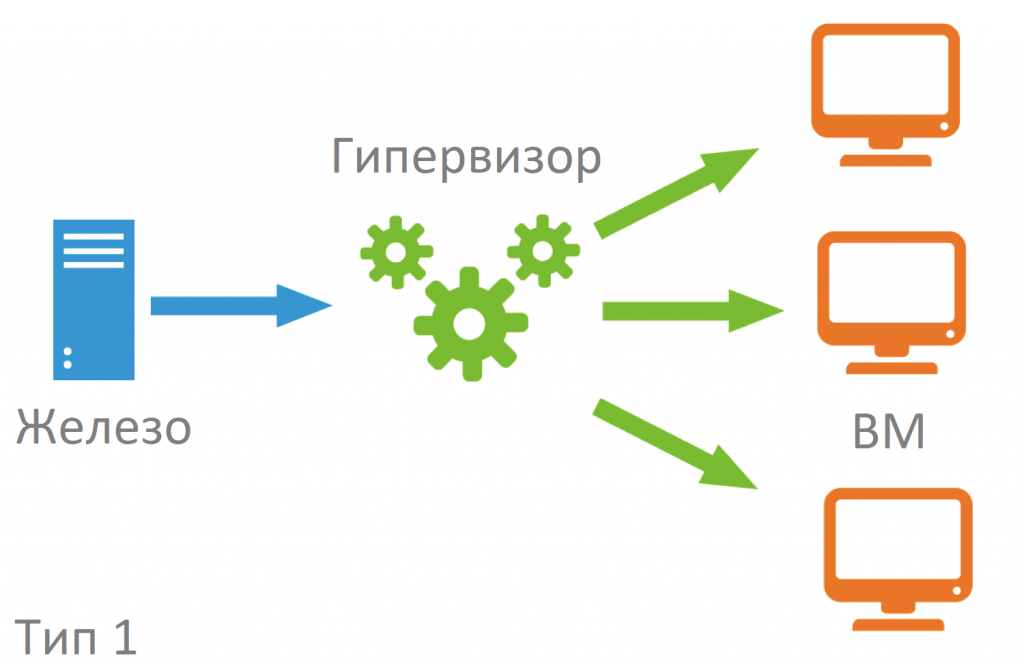
\includegraphics[scale = 0.3]{images/type1.png}
	\caption{Схема гипервизора первого типа}
\end{figure}

\par Для реализации взаимодействия между операционными системами на основе гипервизора первого типа предлагается выполнить установку двух виртуальных машин. На каждую из виртуальных машин необходимо установить соответствующую операционную систему - Android и Linux Debian. Операционные системы смогут коммуницировать между собой используя гипервизор. В свою очередь гипервизор будет взаимодействовать с аппаратной частью устройства при необходимости. Таким образом две операционные системы будут обособлены друг от друга, но в тоже время иметь возможность обмениваться информацией по средствам гипервизора.

\clearpage

\subsubsection{Архитектруа на основе гипервизора второго типа}

\par Гипервизоры второго типа, иногда называемые «хостовыми гипервизорами», запускаются на обычной операционной системе, как и другие приложения в системе. В этом случае гостевая ОС выполняется как процесс на хосте, а гипервизоры разделяют гостевую ОС и ОС хоста. Примеры гипервизоров второго типа:
\begin{itemize}
    \item VMware Workstation
    \item VMware Player
    \item VirtualBox
    \item Parallels Desktop для Mac
\end{itemize}

\begin{figure}[h!]
	\centering
	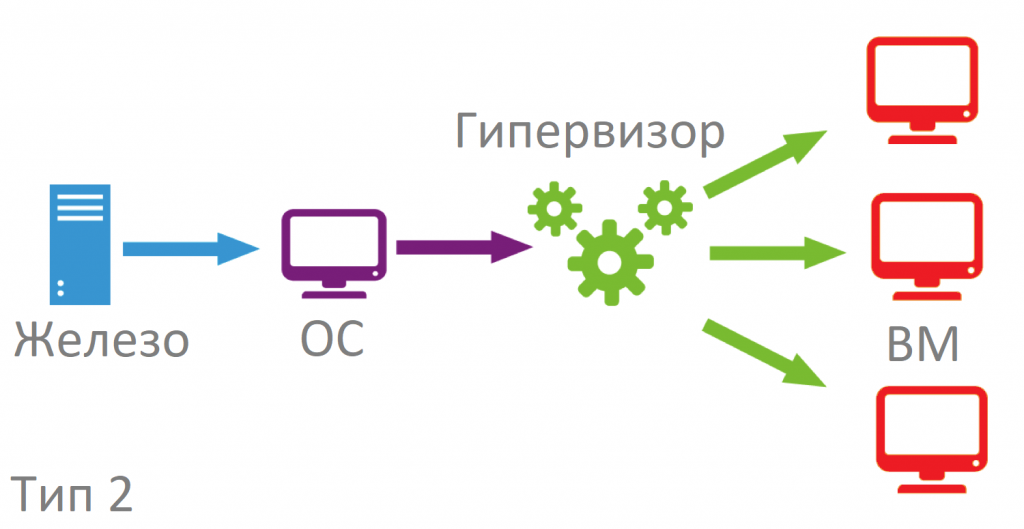
\includegraphics[scale = 0.3]{images/type2.png}
	\caption{Схема гипервизора второго типа}
\end{figure}

\par Для реализации взаимодействия между операционными системами на основе гипервизора второго типа предлагается установить Android - в качестве операционной системы, которая будет взаимодействовать с аппартной частью устройства, а также отправлять информацию через гипервизор. Linux Debian предлагается поставить на виртуальную машину, у которой будет возможность взаимодействовать с реальной опреационной системой с помощью гипервизора. Таким образом получится полноценный Android и Linux на виртуальной машине. При необходимости взаимодействия Linux'а с аппаратной частью, будет отправляться соответствующий вызов в гипервизор, который перешлёт данный вызов далее в Android, в свою очередь из которого будет выполнено взаимодействие с аппаратной частью.  

\subsection{Android API}
\par Так как в MARU OS используется две отдельных операционных системы. Следовательно в MARU используются стандартные вызовы соответствующих операционных систем. Поэтому ниже представлена часть определний, которые содержаться в части андроида на репозитории MARU OS:

\textbf{Networking}

\begin{itemize}
    \item android\_getaddrinfofornetwork(net\_handle\_t network, const char *node, const char *service, const struct addrinfo *hints, struct addrinfo **res)
    \item android\_res\_cancel(int nsend\_fd)
    \item android\_res\_nquery(net\_handle\_t network, const char *dname, int ns\_class, int ns\_type, uint32\_t flags)
    \item android\_res\_nresult(int fd, int *rcode, uint8\_t *answer, size\_t anslen)
    \item android\_res\_nsend(net\_handle\_t network, const uint8\_t *msg, size\_t msglen, uint32\_t flags)
    \item android\_setprocnetwork(net\_handle\_t network)
    \item android\_setsocknetwork(net\_handle\_t network, int fd)
\end{itemize}

\textbf{Memory}

\begin{itemize}
    \item ASharedMemory\_create(const char *name, size\_t size)
    \item ASharedMemory\_dupFromJava(JNIEnv *env, jobject sharedMemory)
    \item ASharedMemory\_getSize(int fd)
    \item ASharedMemory\_setProt(int fd, int prot)
\end{itemize}

\textbf{Storage}

\begin{itemize}
    \item AObbInfo\_delete(AObbInfo *obbInfo)
    \item AObbInfo\_getFlags(AObbInfo *obbInfo)
    \item AObbInfo\_getPackageName(AObbInfo *obbInfo)
    \item AObbInfo\_getVersion(AObbInfo *obbInfo)
    \item AObbScanner\_getObbInfo(const char *filename)
    \item AStorageManager\_delete(AStorageManager *mgr)
    \item AStorageManager\_getMountedObbPath(AStorageManager *mgr, const char *filename)
    \item AStorageManager\_isObbMounted(AStorageManager *mgr, const char *filename)
    \item AStorageManager\_mountObb(AStorageManager *mgr, const char *filename, const char *key, AStorageManager\_obbCallbackFunc cb, void *data)
    \item AStorageManager\_unmountObb(AStorageManager *mgr, const char *filename, const int force, AStorageManager\_obbCallbackFunc cb, void *data)
\end{itemize}

\textbf{Camera}

\begin{itemize}
    \item ACameraCaptureSession\_abortCaptures(ACameraCaptureSession *session)
    \item ACameraCaptureSession\_capture(ACameraCaptureSession *session, ACameraCaptureSession\_captureCallbacks *callbacks, int numRequests, ACaptureRequest **requests, int *captureSequenceId)
    \item ACameraCaptureSession\_close(ACameraCaptureSession *session)
    \item ACameraCaptureSession\_getDevice(ACameraCaptureSession *session, ACameraDevice **device)
    \item ACameraCaptureSession\_logicalCamera\_capture(ACameraCaptureSession *session, ACameraCaptureSession\_logicalCamera\_captureCallbacks *callbacks, int numRequests, ACaptureRequest **requests, int *captureSequenceId)
    \item ACameraCaptureSession\_logicalCamera\_setRepeatingRequest(ACameraCaptureSession *session, ACameraCaptureSession\_logicalCamera\_captureCallbacks *callbacks, int numRequests, ACaptureRequest **requests, int *captureSequenceId)
    \item ACameraCaptureSession\_setRepeatingRequest(ACameraCaptureSession *session, ACameraCaptureSession\_captureCallbacks *callbacks, int numRequests, ACaptureRequest **requests, int *captureSequenceId)
    \item ACameraCaptureSession\_stopRepeating(ACameraCaptureSession *session)
    \item ACameraCaptureSession\_updateSharedOutput(ACameraCaptureSession *session, ACaptureSessionOutput *output)
\end{itemize}

\subsection{Linux API}

\par Системные вызовы могут быть сгруппированы в пять больших категорий:

\begin{enumerate}
\item \textbf{Управление процессами}

\begin{itemize}
    \item load
    \item execute
    \item end (exit), abort
    \item создание процесса (fork в Unix-like, NtCreateProcess в Windows\_NT Native API)
    \item завершение процесса
    \item get/set process attributes
    \item wait время, события, signal события
    \item allocate, free memory
\end{itemize}

\item \textbf{Работа с файлами}

\begin{itemize}
    \item create file, delete file
    \item open, close
    \item read, write, reposition
    \item get/set file attributes
\end{itemize}

\item \textbf{Управление устройствами}

\begin{itemize}
    \item request device, release device
    \item read, write, reposition
    \item get/set device attributes
    \item logically attach or detach devices
\end{itemize}

\item \textbf{Работа с информацией}

\begin{itemize}
    \item get/set time or date
    \item get/set system data
    \item get/set process, file, or device attributes
\end{itemize}

\item \textbf{Связь, коммуникация}

\begin{itemize}
    \item create, delete communication connection
    \item send, receive messages
    \item transfer status information
    \item attach or detach remote devices
\end{itemize}

\end{enumerate}

\par В данном разделе представлена малая часть системных вызовов.

\textbf{sys\_futex}

\par Системный вызов sys\_futex обеспечивает программный метод для ожидания изменения значения указанного адреса памяти и метод пробуждения всех ожидающих на определенном адресе (хотя адреса для одного и того же участка памяти в разных процессах могут быть не идентичны, ядро распределяет их внутренне так, что один участок памяти, распределенный разными методами, будет соответствовать одинм вызовам sys\_futex). Обычно это используется для реализации случаев споров за блокировку разделяемой памяти, как это описано в futex(4).

\par Когда операции futex(4) заканчиваются без завершения спора в пространстве пользователя, должен быть сделан вызов к ядру для выноса решения. Вынос решения может означать как усыпление вызывающего процесса, так и наоборот - пробуждение ожидающего процесса.

\par Вызывающие эту функцию должны твердо придерживаться семантики, описанной в futex(4). Так как эта семантика приводит к созданию непортируемых инструкций ассемблера, то фактически это приведет к тому, что большинство использующих их пользователей станут авторами библиотек, а не создателями программ.

\par Аргумент futex должен указывать на выровненное целое, хранящее счетчик. Операция для исполнения передается через параметр op вместе со значением val.

\textbf{epoll\_wait}

\par Системный вызов epoll\_wait() ожидает события на экземпляре epoll(7), на который указывает файловый дескриптор epfd. Область памяти, на которую указывает events, будет содержать события, доступные для вызываемого. Вызов epoll\_wait() может вернуть до maxevents событий. Параметр maxevents должен быть больше нуля.
В аргументе timeout указывается количество миллисекунд, на которые блокируется epoll\_wait()

\textbf{clock\_getres()}

\par Функция clock\_getres() определяет разрешающую способность (точность) заданных в clk\_id часов, и, если res не равно NULL, сохраняет её в struct timespec, указанную в res. Точность часов зависит от реализации и не может быть настроена определённым процессом. Если значение времени, указанное в аргументе tp функции clock\_settime(), не кратно res, то оно усекается до кратного res.
Функции clock\_gettime() и clock\_settime() получают и устанавливают время указанных часов clk\_id.

\textbf{write}

\par write записывает до count байтов из буфера buf в файл, на который ссылается файловый описатель fd. POSIX указывает на то, что вызов write(), произошедший после вызова read() возвращает уже новое значение. Заметьте, что не все файловые системы соответствуют стандарту POSIX.  \\

\par В случае успешного завершения возвращается количество байтов, которые были записаны (ноль означает, что не было записано ни одного байта). В случае ошибки возвращается -1, а переменной errno присваивается соответствующее значение. Если count равен нулю, а файловый описатель ссылается на обычный файл, то будет возвращен ноль и больше не будет произведено никаких действий. Для специальных файлов результаты не могут быть перенесены на другую платформу.

\textbf{read}

\par read() пытается записать count байтов файлового описателя fd в буфер, адрес которого начинается с buf.
Если количество count равно нулю, то read() возвращает это нулевое значение и завершает свою работу. Если count больше, чем SSIZE\_MAX, то результат не может быть определен. 

\par При успешном завершении вызова возвращается количество байтов, которые были считаны (нулевое значение означает конец файла), а позиция файла увеличивается на это значение. Если количество прочитанных байтов меньше, чем количество запрошенных, то это не считается ошибкой: например, данные могли быть почти в конце файла, в канале, на терминале, или read() был прерван сигналом. В случае ошибки возвращаемое значение равно -1, а переменной errno присваивается номер ошибки. В этом случае позиция файла не определена

\textbf{mmap}

\par Функция mmap отражает length байтов, начиная со смещения offset файла (или другого объекта), определенного файловым описателем fd, в память, начиная с адреса start. Последний параметр (адрес) необязателен, и обычно бывает равен 0. Настоящее местоположение отраженных данных возвращается самой функцией mmap, и никогда не бывает равным 0.
Аргумент prot описывает желаемый режим защиты памяти (он не должен конфликтовать с режимом открытия файла). Оно является либо PROT\_NONE либо побитовым ИЛИ одного или нескольких флагов PROT\_*.


\end{document}